\documentclass[12pt,oneside]{memoir}

\usepackage[biblatex]{matfmaster}
\usepackage{listings}

\bib{master}

\autor{Милош Самарџија}
\naslov{Развој микросервисне апликације за Android коришћењем окружења Lumen}
\godina{2021}

\mentor{др Милена \textsc{Вујошевић Јаничић}, доцент\\ Универзитет у Београду, Математички факултет}
\komisijaA{др Филип \textsc{Марић}, ванредни професор\\ Универзитет у Београду, Математички факултет}
\komisijaB{др Александар \textsc{Картељ}, доцент\\ Универзитет у Београду, Математички факултет}

% \datumodbrane{ }

% \apstr{ }

\kljucnereci{микросервиси, рачунарство, развојни оквир, андроид, трчање}

\begin{document}

\frontmatter
\naslovna
\komisija
% \posveta{Мојој породици}
% \apstrakt
\tableofcontents*

\mainmatter

\chapter{Увод}
Микросервисна архитектура представљa популаран приступ развоју скалабилних дистрибуираних система. Главна филозофија на којој је овај приступ заснован је доменски оријентисано моделовање (енг.~\textit{domain-driven design}), које подстиче разбијање комплексних домена на што једноставније и независније поддомене.

Главна тематика којом се овај рад бави су основне идеје водиље доменски оријентисаног моделовања, начин на који их микросервисна архитектура инкорпорира, као и дизајн REST (енг.~\textit{representational state transfer}) интерфејса за програмирање апликација (енг.~\textit{RESTful API}) који представљa једну од техника за интеграцију поддомена система. У те сврхе је осмишљенa и развијена апликација чији је циљ да илуструје примену микросервисне архитектуре у пракси, као и комуникацију са екстерним сервисима.

Апликација је названа \textit{My Running Buddy}, а њена примарна намена је проналажење партнера за трчање на основу различитих параметара. Сам алгоритам за упаривање тркача уједно представљa и најважнији поддомен (енг.~\textit{core subdomain}) целог система, и на њега је потребно обратити највише пажњe током дизајна и имплементације. Део апликације је написан у програмском језику PHP коришћењем Lumen развојног оквира за развој микросервисних апликација и REST интерфејса за програмирање апликација, где је највећи део доменске логике садржан. Други део апликације је написан у програмском језику Java, заједно са Android комплетом за развој софтвера (енг.~\textit{Android SDK}) и представља кориснички интерфејс, односно улазну тачку у систем. За потребе складиштењa података од стране микросервиса користи се база података MySQL.

У поглављу \ref{domenskiorijentisanomodelovanje} се обрађује доменски оријентисано моделовање, односно, основни концепти, циљеви и препоруке филозофије. Разумевање овог поглавља је кључно за разумевање сврхе микросервиса, на који начин се систем разбија на сервисе и колика грануларност тих сервиса треба да буде. Микросервисна архитектура није први и једини архитектурални стил који је увео декомпозицију система на сервисе; без разумевања идеологије коју заступа, тешко би било уочити разлику између микросервиса и било које друге сличне архитектуре. Поглавље \ref{mikroservisi} успоставља везу између микросервиса и доменски оријентисаног моделовања, анализира најважније предности и мане оваквог дизајна, и обрађује теме везане за упошљавање микросервиса и њихово тестирање. Поглавље \ref{prakticnideo} укратко даје преглед технологија употребљених у пројекту, описује процес креирања апликације, од фазе планирања и дизајна, па све до најбитнијих имплементационих детаља и изазова. На крају, у последњем поглављу, изведен је закључак где су сумирани доприноси, и утисци стечени током израде рада.

\chapter{Доменски оријентисано моделовање}\label{domenskiorijentisanomodelovanje}
Доменски оријентисано моделовање је филозофија развоја чији циљ је управљање конструкцијом и одржавањем софтвера писаног за комплексне домене \cite{DomainDrivenDessign}. Циљ се достиже употребом одређених образаца (енг.~\textit{patterns}), принципа и добрих пракси које, уколико се добро разумеју и примене, смањују шансу за прављење неких честих грешака које се јављају током развоја.

\section{Идеја филозофије и основни концепти}
Идеја водиља ове филозофије је разбијање великих и комплексних домена на једноставније поддомене. Ово има двојаки значај:
\begin{enumerate}
\item добијамо поддомене који су мање комплексни, и који имају јаснију одговорност
\item лакше се проналазе и изолују најважнији поддомени у које је потребно уложити највећи део времена, јер је то оно што одређени софтвер чини другачијим од осталих решења, и представља разлог због којег је уопште и настао
\end{enumerate}

Такође, филозофија инсистира на томе да се у пројекат активно укључе и доменски експерти (енг.~\textit{domain experts}) чија би примарна улога била упознавање програмера и остатка тима са комплексним доменом како би се избегле недоумице и погрешна решења. Ово функционише тако што се током целог развојног циклуса организују формални и неформални састанци са експертима, где се кроз дискусију и различите активности (енг.~\textit{knowledge crunching}) врши анализа и разбијање домена на више мањих, и моделовање поддомена. Као пропратни ефекат ових састанака настају аналитички модел, и заједнички језик (енг.~\textit{ubiquitous language}) чија је улога избегавање двосмислености у комуникацији између експерата и програмера. Током животног циклуса пројекта разумевање домена постаје боље, а заједно са разумевањем се развијају и расту заједнички језик и модели. Сва комуникација, модели и кôд су изражени у терминима заједничког језика.

\subsection{Чести проблеми развоја комплексних апликација}
Да бисмо разумели сврху постојања ове филозофије, потребно је да разумемо на какве изазове се најчешће наилази током развоја и одржавања софтвера. Један од популарнијих архитектуралних стилова коришћених у комплексним апликацијама је тзв. велика лопта од блата (енг.~\textit{Big Ball of Mud}) коју карактерише лош дизајн кôда са одсуством било какве организације. Такав софтвер је углавном доста спрегнут, и захтев за променом једне од функционалности може изазвати ланчану реакцију других измена које нису планиране, али су у том случају неопходне. Проблем је то што није лако уочљиво када пројекат скрене са правог пута, и од добре архитектуре дође до велике лопте од блата. Временом се софтвер инкрементално квари, додавањем нових функционалности, и крпљењем постојећих, уз слабу бригу о одржању архитектуре, са изговором да ће некад касније бити издвојено време за рефакторисање. Тако настаје технички дуг (енг.~\textit{technical debt}).

Технички дуг је концепт у развоју софтвера настао као еквивалент новчаног дуга. Суштина концепта је да, занемаривањем дизајна кôда, дуг постаје све већи, и све је мање вероватно да ће бити успешно измирен. У преводу, долази се до стадијума када је свака измена спецификације (која даље повлачи измене у кôду) болна јер је софтвер постао изузетно спрегнут, и много компоненти зависи од других, иако у природи можда чак и не постоји таква веза између тих ентитета. Немогуће је направити изоловане измене, већ су оне раштркане широм система, и због тога се веома лако могу увести нове грешке (енг.~\textit{bugs}) у систем.

Јасно је да су измене спецификације неизбежне, па нам једино преостаје да се прилагодимо; у супротном, велика је вероватноћа да ће пројекат бити неуспешан, делимично функционалан и/или тежак за одржавање. У тој ситуацији се, у зависности од тренутног стања кôда, долази до закључка да је неопходно извршити опширно рефакторисање, или дизајнирање и писање софтвера испочетка. То све доводи до већих трошкова развоја, који су се могли избећи.

\subsection{Аналитички модел}
Аналитички модел је колекција артефаката који описују модел система, и намена му је да програмерима и пословним корисницима помогне да боље разумеју домен \cite{DomainDrivenDessign}. Да би овај модел био користан, све време мора бити усклађен са имплементационим моделом, тј. измене у имплементацији се морају огледати у изменама у аналитичком моделу, и обрнуто. Ова усклађеност постиже се управо изражавањем оба модела у терминима заједничког језика.

Да би се ово остварило, имплементациони модел мора да буде ослобођен било каквих брига које су техничке природе, и да буде фокусиран искључиво на домен. Такође, битно је да аналитички модел буде једноставан за имплементацију, тј. да не буде превише апстрактан, или на превише високом нивоу. Пројекти који постану тешки за одржавање управо пате од недостатка фокуса на домен; технички проблеми бивају помешани са доменском логиком, и дизајн кôда се везује за техничке појмове, уместо за домен. То доводи до повећања сложености, и отежаног разумевања пројекта од стране нетехничких лица попут доменских експерата. Комуникација се успорава услед велике количине времена утрошеног на објашњавање техничких концепата нетехничким лицима, врло лако долази до неразумевања и јављају се двосмислености, а потом настају и погрешна софтверска решења.

\subsection{Врсте поддомена}
Разбијањем комплексног домена открива се више мањих и једноставнијих поддомена са мањим бројем одговорности. Сваки од поддомена се може сврстати у неку од категорија: главни, генерички (енг.~\textit{generic}) и потпорни (енг.~\textit{supporting}) поддомени. Уз сваки добијени поддомен се придружује његов одговарајући модел.

Под генеричким поддоменима се подразумевају неке од најраспрострањенијих функционалности које и већина других система такође има. Један пример генеричког поддомена може бити подсистем за слање и примање порука. Ово наравно не мора увек бити тачно. Генерички поддомен једног система може бити главни поддомен унутар другог система. У нашем примеру са подсистемом за поруке, у већини система ће вероватно бити сврстан као генерички, али ће представљати главни поддомен у системима чији је највећи адут управо размена порука.

У потпорне поддомене спадају све остале ствари које представљају подршку за функционисање главних домена. Заједничка ствар за потпорне и генеричке домене је то што су у односу на главне поддомене мање битни, али су неопходни јер без њих систем не може бити комплетан.

Главни поддомен садржи највећи и најбитнији део доменске логике, и у зависности од његовог модела и одговарајуће имплементације зависи да ли ће софтвер бити популаран и добро прихваћен, или ће се придружити великом броју других осредњих софтверских решења. Спецификација главног поддомена ће бити најподложнија изменама, и дизајнирању његовог модела треба приступити пажљиво, како би био довољно флексибилан да подржи све накнадне измене. Моделовани систем може садржати и више од једног главног поддомена уколико се врши декомпозиција проблема са изузетно комплексним доменом.

Са друге стране имамо потпорне и генеричке поддомене чији дизајн може бити слободнији, па се чак могу користити и неке готове софтверске библиотеке (енг.~\textit{third party libraries}). С обзиром да њихов модел не мора бити превише флексибилан, и највероватније ће трпети најмање измена, могло би да се толерише и да се неки од њих временом претвори у велику лопту од блата. Кључно је то што је тај лош дизајн изолован од остатка система, и онемогућено му је даље ширење. Уместо претераног фокусирања на потпорне и генеричке поддомене, може се уложити додатни труд у развој главног поддомена. Програмери са мање искуства могу бити задужени за потпорне и генеричке поддомене, а они искуснији могу да се преусмере на главне поддомене.

\subsection{Доменски модел}
Доменски модел је централни појам доменски оријентисаног моделовања. На почетку се формира у виду аналитичког модела кроз заједничку сарадњу развојног тима и доменских експерата. Не осликава домен у потпуности онако како изгледа у реалности, већ представља поглед на домен из једног угла, односно његову апстракцију, која је довољно добра за случајеве употребе које софтверско решење треба да имплементира. Слика \ref{fig:domenmodelprojekcija} приказује разлику између реалности и самог модела. Модел је описан заједничким језиком којим тим говори, као и дијаграмима које је тим креирао. Садржи само оно што је неопходно у контексту апликације која се креира, и мора да се развија паралелно са пословањем како би био користан и валидан. Модел је користан онолико колико је у стању да представи комплексну логику која решава доменске проблеме, а не колико добро осликава реалност.

Креирање доменског модела није једноставан посао, и представља итеративан процес. Велика је вероватноћа да први добијени модел неће бити задовољавајући, и то не треба да буде обесхрабрујуће. Тим би, заједно са доменским експертима, требало да настави са активностима, у циљу проналажења бољих модела. Не треба се задржати на само једном добром, већ треба пронаћи више задовољавајућих модела. Анализом доменских случајева употребе може се оценити корисност креираног модела, и потврдити да сви чланови тима разумеју домен.

Систем који се конструише се састоји од више целина, где су неке битније од других, па ће постојати и више модела различите сложености који ће се користити у различитим ограниченим контекстима (енг.~\textit{bounded contexts}). С обзиром на захтевност овог процеса, комплексни и богати модели се креирају само за битне поддомене система. 

\begin{figure}[!ht]
  \centering
  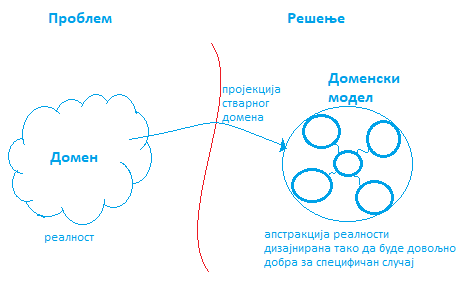
\includegraphics[scale=0.7]{slike/domen-model-projekcija.png}
  \caption{Пројекција реалног домена на једну његову апстракцију}
  \label{fig:domenmodelprojekcija}
\end{figure}
\subsection{Имплементациони обрасци за доменски модел}
Уколико се посматрају слојевите архитектуре софтвера, слој домена би представљао срж апликације. Он изолује сложеност доменског модела од сложености разних техничких делова софтвера. Његова улога је да осигура да се техничке ствари попут логике за управљање трансакцијама, складиштења података и приказивања не умешају у комплексност доменске логике. Мешањем инфраструктурне и доменске логике добија се кôд који је тежи за разумевање, јер има више од једног задужења, и тешко је фокусирати се на само једну ствар. Слој домена обично представља само мали део целокупне апликације, што се може видети на слици \ref{fig:slojevitaarhitektura}.

\begin{figure}[!ht]
  \centering
  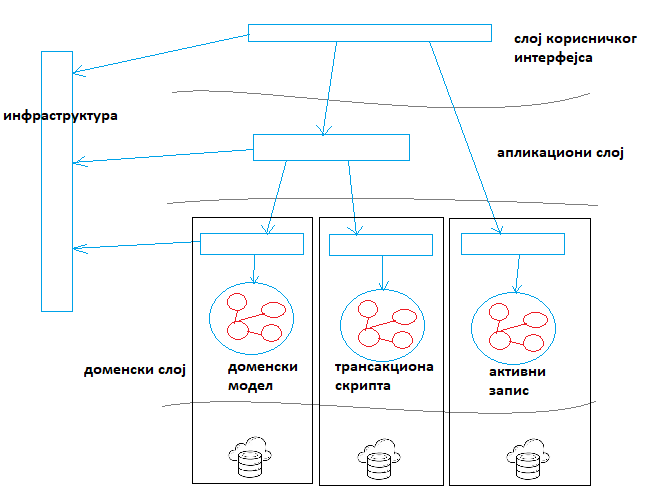
\includegraphics[width=\textwidth]{slike/slojevita-arhitektura.png}
  \caption{Слој домена као део сложеније архитектуре}
  \label{fig:slojevitaarhitektura}
\end{figure}

Конструкција доменских модела је проблем који нема јединствено решење, али у пракси постоје одређена решења, односно имплементациони обрасци, који су општеприхваћени и углавном су се добро показали. Неки од њих више одговарају сложенијим поддоменима, док се други могу искористити код једноставнијих, за прављење простијих и сиромашнијих модела. Популарнији обрасци који се користе су доменски модел (енг.~\textit{domain model}), трансакциона скрипта (енг.~\textit{transaction script}) и активни запис (енг.~\textit{active record})\cite{peaa}.

\paragraph{Образац "доменски модел"}
Овај образац се најбоље уклапа у комплексне домене са богатом пословном логиком, и подразумева креирање објектно-оријентисаног модела који садржи податке, пословне процесе и правила, и богату доменску логику. Премиса обрасца је да не постоји база података, и да током еволуирања модела проблем складиштења података буде занемарен. Објекти у добијеном моделу су у потпуности ослобођени од инфраструктурних проблема, што омогућава да дизајн модела буде фокусиран искључиво на домен. На слици \ref{fig:razdvajanjedomenskogsloja} се може видети како је доменски слој раздвојен од техничких ствари попут складиштења података.

\begin{figure}[!ht]
  \centering
  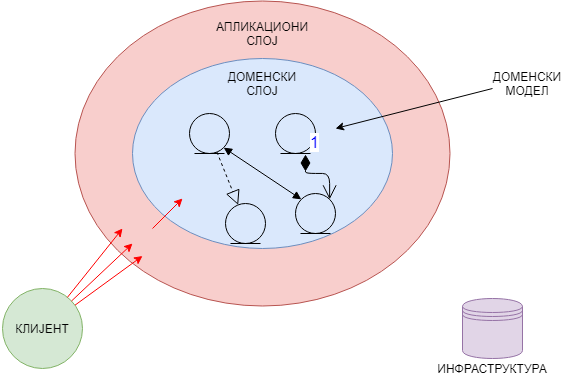
\includegraphics[scale=0.7]{slike/razdvajanje-domenskog-sloja.png}
  \caption{Раздвајање доменског слоја од остатка апликације}
  \label{fig:razdvajanjedomenskogsloja}
\end{figure}

\paragraph{Образац "трансакциона скрипта"}
Трансакциона скрипта је, за разлику од доменског модела, заснована на процедуралном стилу развоја, лакша је за разумевање и имплементацију. Идеја је да се за сваки случај употребе креира по једна процедура, и да се све те процедуре групишу на једно место. Свака од процедура треба да садржи сву логику потребну да се обави одговарајући случај употребе, укључујући ствари попут пословних правила, логике за складиштење података, итд. Предност овог обрасца су једноставност и могућност да се лако имплементирају нови случајеви употребе додавањем нове процедуре, без бојазни да ли ће бити утицаја на постојећу функционалност. Мане су, очигледно, потенцијално много понављања исте логике на различитим местима и лоша подела одговорности. Овакав образац је најприхватљивији за једноставније поддомене који садрже мало логике.

\paragraph{Образац "активни запис"}
Активни запис је популарни образац који подразумева да се сваки објекат модела пресликава у одговарајући ред неке табеле. Погодан је у случајевима када модел базе података одговара доменском моделу. Ова структура ће у себи садржати податке и понашање, као и додатне методе за складиштење, додавање нових инстанци и претраживање колекције објеката. С обзиром да свака од структура има методе за креирање, читање, ажурирање и брисање, могуће је коришћење алата и скриптова за аутоматско генерисање доменског модела.

\subsection{Ограничени контексти и интегритет доменских модела}\label{ogranicenikonteksti}
Већ је поменута битност разбијања главног домена на неколико мањих. Као резултат тог процеса настају једноставнији поддомени са бољом поделом одговорности, и њихови одговарајући модели; како би се остварила функционалност система, неопходно је да постоји нека интеракција између тих модела. Кључно је да модели буду што независнији, и да ова интеракција буде добро дефинисана. У супротном, лако долази до преплитања концепата и логике из различитих поддомена. Да би се заштитио интегритет модела, дефинишу се јасне границе између различитих модела, а то се постиже везивањем модела за одређени контекст, тзв. ограничени контекст.

За разлику од поддомена, који је апстрактан појам, ограничени контексти представљају конкретну техничку имплементацију која ће форсирати одржање граница између модела апликације. Имплементирају се тако да поседују читав стек (енг.~\textit{stack}) функционалности једног поддомена, укључујући презентациони слој, доменску логику и инфраструктуру. Избор архитектуралног обрасца, па и самих технологија за имплементацију једног контекста се може разликовати од контекста до контекста. Сама филозофија не ограничава избор архитектуре, али је потребно да она буде у стању да изолује доменску логику, јер ће се презентација, инфраструктура и доменска логика мењати различитим интезитетом, и из различитих разлога. Један од архитектуралних образаца који омогућава ову изолацију је слојевита архитектура, описана у секцији \ref{sectionslojevitaarhitektura}.

Контексти се дефинишу на начин који би омогућио поделу послова између различитих тимова, и тако да унутар једног контекста нема двосмислених појмова који би увели забуну. Природно је да за један ограничени контекст буде задужен само један тим, унутар којег би се развијао заједнички језик. С обзиром да су ограничени контексти доста независни, и комуникацију са другим контекстима обављају преко јасно дефинисаних интерфејса, један тим би јако мало зависио од других тимова, и њихови рокови дистрибуције нових верзија софтвера не би зависили од другог тима и њихових проблема. Ово важи све док се не наруши компатибилност променом интерфејса преко којих се комуникација обавља.

\section{Слојевитe архитектурe}\label{sectionslojevitaarhitektura}
У претходној секцији је речено да архитектурални стил сваког појединачног ограниченог контекста мора да подржи раздвајање доменске логике од осталих делова, односно раздвајање одговорности. Да би се ово постигло, могу се креирати различити слојеви у оквиру ограниченог контекста, где би сваки слој био задужен за неку од одговорности. На слици \ref{fig:inverzijazavisnosti} се може видети слојевита архитектура са доменским слојем у самом језгру. Доменски слој је у потпуности ослобођен било каквих зависности, и фокусиран је искључиво на доменску логику. Апликациони слој који окружује доменску логику има улогу да имплементира случајеве употребе, и то тако што ће оркестрирати доменским моделима и делегирати захтеве доменском слоју. Једина зависност коју апликациони слој треба да има је зависност од доменског слоја.

Јасно је да ће ова два слоја имати потребу за складиштењем података, и за разним другим инфраструктурним услугама. Да би се ово остварило без увођења додатне зависности, примењује се принцип познатији као инверзија зависности (енг.~\textit{dependency inversion}). Инверзија зависности у овом случају подразумева да, уместо да се апликациони слој прилагођава специфичностима сваке инфраструктурне услуге, свака од услуга имплементира унапред дефинисан интерфејс од стране апликационог слоја. Пропратни ефекат независности апликационог и доменског слоја од остатка је њихово олакшано тестирање, тј. тестирање доменске логике у изолацији, без инфраструктурних зависности.
\begin{figure}[!ht]
  \centering
  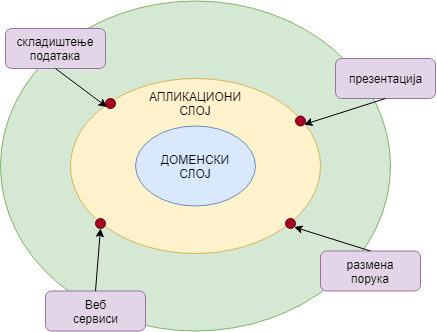
\includegraphics[scale=0.7]{slike/inverzija-zavisnosti.png}
  \caption{Слојевита архитектура апликације са инверзијом зависности}
  \label{fig:inverzijazavisnosti}
\end{figure}
\section{Интеграција ограничених контекста}\label{integracijaogranicenihkonteksta}
Сваки од ограничених контекста може представљати засебан процес који може бити извршаван на различитим физичким машинама. Добра ствар овог приступа где су различити контексти засебни процеси је то што је апликација отпорнија на отказивање одређених компоненти система, па чак и на саме физичке кварове. Додатно, софтвер је скалабилнији. У случају повећаног броја корисника, а самим тим и количине операција који се обрађује од стране апликације, софтвер мора бити у стању да се скалира како би успешно опслужио све кориснике.

Једно од решења је вертикално скалирање, које подразумева повећање хардверских ресурса на једној машини, попут радне меморије, складиштног простора, и броја процесора. Јасно је да овај приступ има ограничење, и да повећање ресурса на тај начин не може бити дугорочно решење. Боље решење је да апликација буде способна да се скалира хоризонтално, односно, да се са порастом оптерећења система додају нове физичке машине у инфраструктуру, и да се покрећу додатне инстанце софтвера. Међутим, по правилу су овакви системи доста сложенији; уместо једне монолитне апликације постоји више дистрибуираних процеса који међусобно морају да сарађују и комуницирају, најчешће посредством рачунарске мреже. Потребно је дефинисати на који начин ће те компоненте бити интегрисане, како ће се синхронизовати, а јавља се и питање конзистентности. Сви наведени проблеми представљају нешто са чиме се сваки дистрибуирани систем суочава, и од система до система се могу разликовати реализована решења, а у зависности од случајева употребе, природе самог домена, и очекивања корисника.

Нека од конкретних техничких решења која могу бити употребљена за комуникацију унутар оваквог система су интеграција коришћењем базе података, интеграција помоћу датотека, позив удаљене процедуре (енг.~\textit{remote procedure call}), интеграција коришћењем система за размену порука (енг.~\textit{messaging}) и REST интерфејси за програмирање апликација.

\subsection{Интеграција коришћењем базе података}
Интеграција коришћењем базе података представља најједноставнији вид интеграције ограничених контекста који подразумева да једна компонента упише нешто у базу података, а да онда друга компонента то прочита. Ово читање би могло да буде имплементирано тако да компонента која чита врши читање на сваких неколико секунди или минута. Иако није захтевно за имплементацију, ово решење поседује и неке мане због којих је прихватљиво употребити га само у некритичним деловима система или у првобитним итерацијама. Неки од проблема који се јављају код оваквог типа интеграције је то што су компоненте спрегнуте са базом података. Уколико једна компонента има захтев за променом схеме базе података, друга компонента би морала да се прилагоди тој новој схеми. Такође, код база података као потенцијални проблем се јавља и закључавање које се поприлично може одразити на перформансе уколико један део апликације нпр. интезивно уписује у базу, а други део врши ажурирање. Поред тога, код овакве интеграције база је критична тачка пуцања. Уколико база није доступна, комуникација између компоненти ће бити онемогућена. 

\subsection{Интеграција помоћу датотека}
Овај тип интеграције је доста сличан интеграцији коришћењем базе података. Уместо да део апликације податке уписује у базу података, може их уписати у неку датотеку, из које касније друга компонента може да чита. Овакво решење је некад пожељније у односу на претходно, посебно уколико би апликација базу података користила искључиво за интеграцију. Уместо конфигурисања базе података, у том случају је једноставније податке размењивати преко неке датотеке. Овакав приступ нема проблема са закључавањем, али ипак не нуди решење за скалирање, што значи да би приликом имплементације таквог решења требало осмислити неки механизам за скалирање, редудантност, као и формат самих датотека.

\subsection{Позив удаљене процедуре}
Позив удаљене процедуре је популаран и често коришћен начин интеграције. У основи, комуникација између две компоненте се обавља посредством рачунарске мреже, коришћењем неког протокола, најчешће HTTP. Идеја је да се од програмера прикрије чињеница да су компоненте физички удаљене, и да се комуникација одвија преко мреже. Летимичним погледом на кôд се не може закључити да се ради о мрежној апликацији, јер је сама сложеност мрежне комуникације скривена, а позиви метода, као и њихова имена ни на који начин не откривају да се не ради о монолитној апликацији. У позадини, ово се изводи тако што се за методе које представљају удаљене процедуре генерише клијентски и серверски кôд. Он између осталог садржи логику за серијализацију и десеријализацију параметара и позиве мрежних функција. Позив метода у клијентској апликацији проузрокује да се порука са информацијом о методу који се позива и листом параметара серијализује у низ бајтова, и онда се шаље кроз мрежу. На серверској страни се порука прима, десеријализују се назив метода и његови параметри, и извршава се одговарајући удаљени кôд. Транспарентност овог начина интеграције уједно може бити и његова мана. Врло је лако заборавити да се ради о мрежним позивима, па њихово неоптимално и пречесто позивање може довести до проблема са перформансама. Такође, позиви удаљених процедура су проблематични уколико постоји захтев да се неки кôд извршава асинхроно. У том случају, боље решење представља коришћење система за размену порука.

\subsection{Интеграција коришћењем система за размену порука}
Интеграција коришћењем система за размену порука се користи у апликацијама чије компоненте би требало да комуницирају асинхроно. Систем за размену порука је најчешће имплементиран као дистрибуирани ред који има могућност да се скалира, реплицира податке и шаље их кроз мрежу, и може се посматрати као засебна компонента. У односу на позив удаљених процедура, овај метод интеграције је отпорнији на отказивање компоненти, јер савремени системи за размену порука имају могућност чувања порука које нису послате, у случајевима када постоје мрежни проблеми, или уколико компонента која прима поруке привремено није активна, као и поновно слање тих порука када је систем поново стабилан. Када нека компонента жели да шаље поруке, шаље их у виду догађаја (енг.~\textit{events}), заједно са додатним подацима неопходним за обрађивање тог типа догађаја. Компоненте заинтересоване за одређени тип догађаја се могу претплатити (енг.~\textit{subscribe}) на исти. На овај начин компонента која врши слање уопште не мора да зна ко све прима поруку, већ ће компоненте које желе да обрађују одређени тип догађаја претплатом изразити интересовање. Мана овог приступа је то што се подразумева употреба асинхроне парадигме, која је скоро увек захтевнија за имплементацију и разумевање јер се доста разликује од конвенционалног синхроног програмирања. Такође, захтева посматрање проблема из другачијег угла, као и сасвим другачији дизајн компоненти.

\subsection{REST интерфејси за програмирање апликација}
REST интерфејси су интерфејси за програмирање апликација који су имплементирани у складу са REST архитектуралним стилом и омогућавају комуникацију са удаљеним сервисима. Дизајнирани су тако да могу да искоришћавају постојеће протоколе и због тога није неоподна инсталација додатних библиотека и додатног софтвера. Најчешће се користи HTTP, али у теорији се може користити било који протокол. Неки од критеријума које интерфејс мора да задовољи да би био у складу са REST архитектуралним стилом су:
\begin{enumerate}
\item клијентско-серверска архитектура која се састоји од клијената, сервера и ресурса,
\item комуникација између клијената и сервера је без стања, односно, сервери не чувају информације о клијентима између различитих захтева (непостојање сесије),
\item сваки ресурс мора бити јединствено идентификован, и њихова интерна репрезентација треба бити раздвојена од репрезентације која се шаље клијентима,
\item репрезентација ресурса коју добија клијент мора да садржи довољно информација које ће омогућити манипулацију самим ресурсом, као и довољно информација о томе како би клијент требало да процесира поруку,
\item коришћење хипермедија у одговору који би референцирали друге повезане ресурсе.
\end{enumerate}
Централни појам REST архитектуре је ресурс. Ресурсом се може сматрати практично све што је довољно важно да буде референцирано; то су најчешће ствари које могу бити складиштене у рачунарима, попут електронских докумената, редова у базама података и резултата неког алгоритма. Услов који мора да задовољи сваки ресурс је да има свој јединствени идентификатор URI (енг.~\textit{unique resource identifier}) на основу којег ће бити референциран \cite{RESTfulWebAPIs}. Називи ресурса би требало да буду именице, а не глаголи; у фокусу архитектуре су ресурси, а не процедуре. Добри кандидати за ресурсе су поддомени који су добијени анализом и разбијањем проблема, као и независни ентитети који представљају део модела тих поддомена.

Ресурси се организују логички у хијерархије. Хијерархија се успоставља угњеждавањем имена ресурса у URI идентификатору. Име ресурса који је хијерархијски ниже у односу на неки други ресурс се у јединственом идентификатору појављује касније. Оваквим приступом се јасније осликава однос међу ресурсима; нпр. идентификатор \textit{/knjige/[id knjige]/recenzije/[id recenzije]} јасније говори о односу ентитета "књига" и "рецензија" него два одвојена идентификатора \textit{/knjige/[id knjige]} и \textit{/recenzije/id recenzije}. Други разлог за овакву организацију је зависност неких ресурса од контекста у којем се налазе; у идентификатору \textit{/ulice/[naziv ulice]/kuce/[broj kuce]} број куће је локалан у односу на улицу у којој се налази.

Комуникација међу сервисима се одвија разменом репрезентација ресурса. Битно је напоменути да сам ресурс и његова репрезентација не представљају исту ствар. Репрезентација ресурса је стање ресурса представљено на користан начин, у одређеном формату. Формат који се користи за репрезентацију није дефинисан самим архитектуралним стилом, и може се користити формат по избору. Најчешће се користе JSON (енг.~\textit{JavaScript Object Notation}) и XML (енг.~\textit{eXtensible Markup Language}), због њихове једноставности, флексибилности и доступности великог броја различитих имплементација рашчлањивача (енг.~\textit{parser}).

Поред појединачних ресурса, могуће је конструисати и скупове ресурса истог типа, односно колекцију ресурса. Сама колекција, и сваки од њених елемената има свој јединтвени идентификатор. Дохватањем репрезентације колекције, враћа се листа репрезентација објеката који се у њој налазе. Добра пракса је да се за сваки елемент колекције прикаже мининална репрезентација, уз хипермедиј који ће водити ка детаљној репрезентацији. Такође, требало би омогућити и филтрирање елемената колекције на основу различитих параметара, како би се сузио скуп елемената на неки одређени подскуп. У случају великих колекција, потребно је увести пагинацију којом би се ограничио број елемената који се враћа једним одговором.   

\subsubsection{Креирање захтева}
Манипулација удаљеним ресурсима се врши формирањем захтева у одређеном формату где се наводи јединствени идентификатор ресурса, глагол који описује каква операција се врши над ресурсом, и додатни атрибути који описују остале специфичности које се односе на операцију која се извршава. Операције за манипулацију се могу поделити у две групе: оне које мењају стање ресурса, и оне које не мењају. Мењање ресурса подразумева мењање стања постојећих ресурса, додавање нових и брисање постојећих ресурса.

Уколико се за комуникацију користи HTTP протокол, креирање захтева подразумева попуњавање заглавља и тела HTTP поруке. У заглављу се наводи URL ресурса, а глагол који описује операцију може бити један од предефинисаних глагола у склопу протокола (GET, POST, PATCH, DELETE, PUT). Обрада захтева се имплементира тако да се поштује семантичко значење глагола који се шаље у захтеву. Нпр. GET би било неприродно користити за све осим за дохватање репрезентације ресурса, и било би очекивано да такав захтев не мења стање. Додатне информације које се прослеђују кроз захтев се наводе додавањем HTTP атрибута и попуњавањем тела HTTP поруке.

Семантичка значења HTTP глагола су следећа:
\begin{enumerate}
\item GET - дохвата репрезентацију удаљеног ресурса који је референциран његовим јединственим идентификатором, без мењања стања ресурса.
\item POST - креира нове ресурсе, али се може користити и за акције које мењају стање, али не стварају нове ресурсе.
\item PATCH - мења постојећи ресурс новим ресурсом.
\item DELETE - брише ресурс референциран јединственим идентификатором.
\item PUT - мења стање постојећих ресурса.
\end{enumerate}

\subsubsection{Формат одговора}
Одговор на одређени захтев треба да садржи информацију о статусу извршене операције. Додатно може садржати и репрезентације ресурса, као и хипермедије ка повезаним ресурсима. За статус захтева код HTTP протокола се користе постојећи статусни кодови који су дефинисани стандардом. Као и глаголи, кодови се користе тако да поштују њихово семантичко значење.

\chapter{Микросервисна архитектура}\label{mikroservisi}
Микросервиси представљају архитектурални стил којег одликују мали, независни сервиси који раде заједно како би обавили неки посао. Због сличности, неретко долази до мешања термина микросервиса и доменски оријентисаног моделовања. Та сличност потиче од чињенице да доменски оријентисано моделовање представља само филозофију развоја, односно скуп препорука, образаца и циљева, док су микросервиси једно конкретно решење како се та филозофија може применити у стварности.

Употреба доменски оријентисаног моделовања у микросервисној архитектури се огледа у декомпоновању апликације на мале, добро дефинисане сервисе праћењем смерница за разбијање домена на поддомене, образаца за моделовање добијених поддомена и применом стратегија за интеграцију резултујућих сервиса; ове смернице, обрасци и стратегије су описане у оквиру поглавља \ref{domenskiorijentisanomodelovanje}. Оно што микросервисну архитектуру чини јединственом у односу на друге архитектуралне стилове који такође врше декомпозицију система на сервисе је гранулација сервиса, односно њихова величина, као и оријентисаност сервиса ка домену проблема. Дизајн система моделованог коришћењем доменски оријентисаног моделовања ће садржати ограничене контексте, и управо су ови контексти природне границе сервиса \cite{netmicroservices}. Ограничени контексти су обрађени у секцији \ref{ogranicenikonteksti}.

Скоро сва комуникација се одвија преко мрежних позива, који су скупе операције, и форсира се што већа раздвојеност међу сервисима; на тај начин се смањује опасност од велике спрегнутости. Независност и мала спрегнутост омогућавају да се мењање једног сервиса и дистрибуција нових верзија обављају независно у односу на остале сервисе.

Сваки сервис дефинише интерфејс за програмирање апликација преко којег остали сервиси могу да комуницирају са њим. Раздвојеност сервиса програмерима даје слободу да користе различите програмске језике у различитим сервисима, па технологија која се користи за интерфејс треба да буде језички неутрална (енг.~\textit{language-agnostic}), односно да не ограничава избор програмског језика \cite{BuildingMicroservices}. Поред коришћења различитих програмских језика, различите компоненте такође могу да користе и различите механизме за трајно складиштење података. На пример, један сервис може да буде имплементиран у програмском језику C++ и да користи релациону базу података, а неки други може да буде имплементиран у Пајтону (енг.~\textit{Python}) и да за складиштење користи обичну датотеку. Предност овога је то што се избор технологије може вршити у зависности од природе поддомена и потребних перформанси, преференција особе или тима задуженог за одређени сервис, и слично. Додатно, мање битни сервиси могу да експериментишу са новим технологијама, без страха да ће се евентуални проблеми прелити на остатак система. И наравно, пошто су сервиси мали, врло је лако поново их имплементирати у неком другом програмском језику уколико коришћена технологија не испуни очекивања.   

\section{Предности и мане}
С озбиром да се ради о независним сервисима, јасно је да микросервиси потпадају у категорију дистрибуираних система. Самим тим наслеђују њихове предности и мане. Неке од предности дистрибуираних система су редудантност и отпорност на отказивање, боље скалирање и бржи одзив. Ипак, иако због свега овога звуче као добро решење за сваки проблем, микросервиси имају и отежавајуће околности довољно велике да није исплативо користити их уколико природа самог проблема који се решава не захтева то. Пре свега, ту се мисли на безбедност, проблеме са конзистентношћу и теже детектовање проблема.

\subsection{Редудантност и отпорност на отказивање}
Ова секција започиње поређењем отпорности на отказивање монолитних апликација у односу на микросервисе. Уколико један модул монолитне апликације услед неког проблема откаже, нпр. референцирањем показивача на невалидну меморијску локацију, цела апликација насилно завршава са извршавањем. Такође, ако дође до отказивања физичке машине, једна једина инстанца апликације са којом је корисник имао интеракцију престаје да постоји. Укратко, отпорност на овакве врсте отказа не постоји.

За разлику од монолитне апликације, отказивање једног сервиса у микросервисној архитектури не утиче на доступност осталих сервиса, било да се ради о отказивању сервиса услед неке грешке, или о отказивању физичке машине (ово важи ако се сви сервиси не налазе на истој машини). Један од начина како се микросервисна архитектура бори са оваквим проблемима је да након отказивања систем може да пређе у другачији режим рада, са редукованим функционалностима док се проблематични сервис поново не подигне.

Други начин је постојање резервних (енг.~\textit{backup}) инстанци које би могле да замене инстанцу која више није активна. Резервне инстанце могу бити активне и у стању приправности све време у току рада примарне инстанце, a могу бити и искључене, и покренуте по потреби; то је тзв. хладна резерва (енг.~\textit{cold backup}). Хладна резерва се користи у ситуацијама кад је подизање сервиса брзо, или је период неактивности док се сервис подиже прихватљиво. Предност хладних резерви је у томе што примарни и резервни сервиси нису активни истовремено, па самим тим утрошак ресурса није дупло већи.

Било да се користе активне или хладне резерве, потребно је да постоји механизам који може да утврђује да ли је примарна инстанца активна или није, и да ли је у стању да обрађује захтеве, и да покреће резервне инстанце уколико је потребно. Овај механизам мора радити поуздано, како би се избегла ситуација где и примарна и резервна инстанца активно прихватају и обрађују захтеве; таква ситуација је опаснија од тоталне неактивности, јер може нарушити стање целог система. Једно од софтверских решења које се користи у ове сврхе је Apache ZooKeeper \cite{Zookeeper}.

\subsection{Скалирање}
У секцији \ref{integracijaogranicenihkonteksta} је назначено да постоје два типа скалирања - хоризонтално и вертикално; наведени су и разлози зашто се преферира хоризонтално скалирање у односу на вертикално. Код поддомена који су по природи погодни за паралелизацију постоји могућност покретања више инстанци истог сервиса како би се оптерећење са једне инстанце једнако распоредило на више њих. Број инстанци једног сервиса је динамички, односно, у току већег налета захтева ка систему, покрећу се додатне инстанце како би се избегло оптерећење и успорена обрада података. Када се број захтева врати у нормалу, додатне инстанце се искључују. Ово додавање и избацивање инстанци се може обављати ручно, али може бити и аутоматизовано, тако што ће се број инстанци регулисати на основу статистике, нпр. на основу броја активних корисника, захтева у секунди, одзива и слично. Једна од најбитнијих ствари које корисници система очекују је то да добијају одговоре на њихове захтеве у што краћем року.

\subsection{Одзив}
У претходној секцији је речено да је одзив јако битна карактеристика која може утицати на задовољство корисника. Ово не зависи увек само од оптерећења система, већ и од тога где су корисници географски лоцирани у односу на сам систем. Систем може бити растерећен, али уколико је корисник на другом крају света, спорији одзив услед пропагације података кроз мрежу се не може избећи. Ово се решава тако што се покреће више инстанци истог сервиса, али на различитим локацијама широм света. Балансери захтева на основу локације корисника онда могу да одаберу физички најближи сервис са којим ће корисник комуницирати.

\subsection{Безбедност}
Током развоја софтвера је изузетно битно да се пажња обрати и на безбедност, посебно уколико се ради о софтверу високог значаја \footnote{Ово подразумева софтвер који ради са личним подацима људи, обавља критичне операције које могу утицати на људске животе у економском или здравственом смислу, и било који други софтвер који ради са подацима који се сматрају поверљивим, попут државних тајни, итд.}. Дистрибуирани системи за комуникацију интезивно користе рачунарске мреже, што ствара додатне слабе тачке које је потребно заштитити. Поред стандардних пропуста који се јављају код једнопроцесних апликација, рачунарске мреже отварају нове могућности за искоришћавање система у сврхе које су изван дефинисаних случајева употребе, међу којима су и оне малициозне. Главна линија одбране би требало да буде добро исконфигурисана мрежа која би спречила евентуалне упаде уљеза, али и поред тога, сва комуникација међу сервисима би требало да се одвија као да ће потенцијални уљези пробити заштитну баријеру мреже. То подразумева пажљиво и детаљно обрађивање корисничких захтева; додатно, већина саобраћаја (ако не и сав саобраћај) би требало да буде енкриптована, посебно део комуникације који може садржати осетљиве податке, попут лозинки, бројева картица, и слично.

Код дистрибуираних система код којих су перформансе од великог значаја, посебно код система који раде у реалном времену, енкрипција података може представљати проблем. Криптографске функције могу створити додатни утрошак (енг.~\textit{overhead}) драгоцених ресурса, посебно уколико се користе јачи алгоритми за енкрипцију. У том случају, уместо шифровања свих података у систему, могу се шифровати само осетљиви подаци, као и комуникација између клијената и самог система.

\subsection{Конзистентност}
Постојањем више раздвојених сервиса, добијају се бољи одзив и скалирање, и апликација је отпорнија на отказивање, али се јављају проблеми са конзистентношћу. Конзистентност подразумева да захтев за неким подацима ка било којем сервису унутар система увек враћа најсвежије податке. Пропагација података кроз цео систем захтева одређено време, и јасно је да решење овог проблема не може бити савршено, већ мора постојати неки компромис. Ово тврђење је део познате CAP (енг.~\textit{consistency - availability - partition tolerance}) теореме која каже да је немогуће обезбедити истовремено задовољење конзистентности, расположивости и толеранције раздвојености, и постоји математички доказ који потврђује ову теорему \cite{10.1145/564585.564601}.

\subsection{Надгледање}
Надгледање софтвера (енг.~\textit{monitoring}) у продукцији и детектовање евентуалних проблема је изузетно важан процес. Информациони системи од великог значаја не трпе дуготрајне периоде неактивности, и све потенцијалне проблеме је потребно детектовати на време, и одреаговати што пре. Код монолитних апликација, овај задатак је релативно праволинијски, и подразумева праћење логова, надгледање живости и здравља саме апликације, и то најчешће може бити аутоматизовано. Код микросервиса је ово мало сложеније, због многобројних сервиса које је потребно пратити. Истовремено је потребно пратити стање свих активних инстанци сервиса у систему, на различитим физичким и виртуелним машинама, и овде је аутоматизација неопходна; свако друго решење је непродуктивно. Ручно праћење логова и проверавање појединачних сервиса би захтевало много времена и велики фокус. Додатно, поред здравља појединачних сервиса, потребно је обратити пажњу и на стање мреже која омогућава комуникацију и сарадњу сервиса. Да би се овај задатак аутоматизовао, мора постојати механизам откривања сервиса (енг.~\textit{service discovery}) који може да детектује динамичне промене у инфраструктури, попут додавања нових инстанци и њиховог уклањања.

\section{Упошљавање софтвера}
Упошљавање софтвера (енг.~\textit{deployment}) представља све активности које је неопходно обавити како би се апликација оспособила за употребу. То укључује дистрибуцију нове верзије, инсталацију, конфигурисање, деинсталацију и ажурирања. Ситне промене у комплексним монолитним апликацијама захтевају да се изврши упошљавање целе апликације. Упошљавање велике апликације представља процедуру која носи огроман ризик, па се у пракси овако ризичне процедуре дешавају што је ређе могуће; пре упошљавања се обично скупи доста измена, које се онда дистрибуирају кроз исту верзију. У међувремену су корисници могли да промене мишљење и да одлуче да ипак не желе неку функционалност, или су одлучили да желе да нешто функционише другачије. Услед нагомиланих измена, теже је селективно поништити само неке од измена, посебно јер можда те измене зависе од неких других.

Код микросервиса је прича једноставнија. Сервис у којем су направљене измене се може распоредити независно од осталих сервиса у систему. Лакше се поништавају направљене измене у случају проблема, а и сам проблем је изолован од остатка система. Такође, нове измене се дистрибуирају много брже. Ипак, због постојања више независних сервиса, односно више независних мини пројеката, систем за изградњу (енг.~\textit{build system}) и верзионисање софтвера су комплекснији; додатно, теже је пратити колико инстанци сервиса имамо, и где се све они налазе. Услед непажње, није немогуће заборавити на неки сервис током упошљавања, и зато, ова процедура би требало да буде аутоматизована.

\subsection{Хостовање сервиса}\label{hostovanjeservisa}
Речено је да сваки од сервиса може да се извршава независно, и према томе, сваки од њих се може налазити на различитим машинама. У екстремном случају, сваки сервис може имати своју засебну машину, чиме се постиже велика отпорност на отказивање, и сваки сервис је максимално изолован, с обзиром да су му сви ресурси машине и оперативног система на располагању. Међутим, ово није увек најбоље решење када је у питању искоришћеност ресурса, а притом није ни исплативо; ако се ради о неким једноставним сервисима, ресурси машине ће бити углавном неискоришћени. Уколико желимо велику изолованост сервиса, постоје и друга могућа решења којима се то може постићи.

Једно од класичних решења је употреба виртуелних машина. Једна физичка машина може имати више виртуелних машина, и свака од њих ће имати свој засебан оперативни систем, и у стању је да пружи велики ниво изолације микросервисима. По потреби се могу покретати нове инстанце машина, и гасити постојеће, што даје већу флексибилност него код решења са једном физичком машином по сервису. Ово решење је сасвим прихватљиво, али свака од виртуелних машина хостује по један оперативни систем у целости, и тиме се ствара поприличан додатни утрошак ресурса на гостујуће оперативне системе (енг.~\textit{guest operating system}).

Друго решење је употреба све популарнијих софтверских контејнера, који попут виртуелних машина могу изоловати сервисе од остатка система. И они такође врше одређени степен виртуелизације, али не постоји више инстанци оперативних система, и њихов додатни утрошак је далеко мањи од утрошка који стварају виртуелне машине. Остале предности контејнера у односу на виртуелне машине су:
\begin{enumerate}
\item величина --- с обзиром да контејнери не садрже комплетан оперативни систем, њихова величина се може мерити десетинама мегабајта, што значи да се изузетно брзо могу реплицирати и копирати са једне физичке машине на другу
\item брзина креирања и реплицирања --- због природе контејнера, њихово креирање, реплицирање и уништавање су изузетно ефикасне операције, што погодује великој динамичности дистрибуираних система - могуће је подизање нових инстанци сервиса за свега пар секунди
\end{enumerate}
Један пример технологије софтверских контејнера је Docker \cite{Docker}, који је широко распрострањен у сервисно оријентисаним архитектурама, јер омогућава лако покретање контејнера на инфраструктурама у облаку (енг.~\textit{cloud infrastructure}).

\section{Тестирање}
Тестирање је неизоставан део било које методологије развоја софтвера, и једнако је важно колико и сам процес имплементације. Улога тестирања у развоју је стицање што веће поузданости у исправност софтвера који се развија. Обично није могуће достићи стопроцентну поузданост, али је могуће открити велики број функционалних и нефункционалних недостатака. Од покривености различитих случајева употребе, специјалних случајева и методологије тестирања зависи колико ће тестови добро обављати свој посао. Када говоримо о тестирању микросервиса, једна могућа класификација тестова је на јединичне тестове, тестове појединачних сервиса и тестирање интеграције сервиса, познатије као тестирање са краја на крај (енг.~\textit{end-to-end tests}).

\subsection{Јединично тестирање}
Јединично тестирање подразумева проверу исправности малих логичких целина (обично је то тестирање појединачних функција) од којих је сервис изграђен. Ове логичке целине треба да буду изоловане од остатка сервиса, а све зависности би требало заменити примитивним и лажним (енг.~\textit{mock}) зависностима. Од свих наведених врста тестова, ови тестови су најбржи, требало би да их има највише, и да процентуално детектују највише грешака. Обично су аутоматизовани, и неизоставни су део континуалне интеграције софтвера (енг.~\textit{continuous integration}) која подразумева што чешће "комитовање" (енг.~\textit{commit}) измена, изградњу након сваке измене и покретање аутоматских тестова.

\subsection{Тестирање појединачних сервиса}
Тестирање појединачних сервиса има улогу да провери исправност читавог сервиса, односно функционалности које сервис пружа, и то преко јавног интерфејса који је изложен. Исправност мањих логичких целина је покривена јединичним тестовима, а овај тип тестова би требало да провери да ли су те целине исправно интегрисане. И ове тестове је углавном могуће аутоматизовати. Нешто су спорији од јединичних тестова јер покривају логички веће целине, и количински их има мање.

\subsection{Тестирање са краја на крај}
Претходна два типа тестирања су тестирања која се примењују и код монолитних апликација. Пошто се сервисне архитектуре састоје од више независних компоненти које међусобно сарађују, потребно је увести још један тип тестирања који би проверавао исправност система који се добија интеграцијом припадајућих сервиса. Ово тестирање се примењује тако што се шаљу различити захтеви, који се пропагирају кроз цео систем, а затим се врши анализа исправности добијеног одговора. Ове тестове је могуће делимично аутоматизовати, креирањем скриптова који би се повремено покретали, и њима је могуће тестирати исправност и перформансе система. Ипак, тестирање безбедности целог система није могуће извршити у потпуности аутоматски, већ се тај део посла обавља ручно, и то обично од стране етичких хакера. Тестирање са краја на крај је најспорије и најзахтевније, па је битно да таквих тестова количински нема превише, и да су изабрани тестови квалитетни и репрезентативни.

\chapter{Практични део рада}\label{prakticnideo}
Ово поглавље се односи на практични део рада и представља конкретан пример примене микросервиса. Први део поглавља укратко представља коришћене технологије, а у остатку се описује процес креирања апликације, укључујући планирање, дизајн и фазу имплементације. Овим поглављем биће обухваћене све битније тачке развоја, укључујући изазове и најбитније имплементационе детаље.
\section{Кратак преглед коришћених технологија}
\subsection{Lumen развојни оквир}
Lumen\cite{Lumen} је развојни оквир отвореног кôда за програмски језик PHP, који се користи за развој микросервиса и интерфејса за програмирање апликација. Имплементира MVC (енг.~\textit{model-view-controller}) архитектурлни стил, одликује га велика брзина обраде захтева, и тренутно је најбоље решење, с обзиром да се на тестирању перформанси показао боље у односу на конкурентне развојне оквире попут Silex и Flex 3. Lumen представља олакшану (енг.~\textit{lightweight}) верзију популарног PHP развојног оквира Laravel, односно, дизајниран је тако да буде погодан за развој микросервиса.

Највећа комплексност овог оквира долази управо из Laravel\cite{Laravel} компоненти на које се ослања. Ове компоненте су познатије под именом Illuminate, и имплементиране у складу са унапред дефинисаним интерфејсима, па тако постоје интерфејси за складиштење података, слање мејл порука, и слично. Овај важан принцип је споменут у оквиру секције \ref{sectionslojevitaarhitektura}, где се примењује инверзија зависности како би се избегло увођење инфраструктурних зависности у самој доменској логици. Кључне компоненте су:
\begin{enumerate}
\item компонента за рутирање, чија је улога да све добијене HTTP захтеве повеже са одговарајућом логиком која треба да их обради 
\item компонента средњег слоја (енг.~\textit{middleware}) која се користи за филтрирање захтева који долазе, и на овом слоју се могу радити аутентикација и ауторизација
\item контролер компонента унутар које се налази главна логика апликације (апликациони слој) која оркестрира доменским моделима делегирањем операција
\end{enumerate}

\subsection{Android}
Android\cite{Android} је оперативни систем отвореног кôда који је заснован на модификованој верзији Линукс језгра (енг.~\textit{Linux kernel}), првенствено дизајниран и прилагођен мобилним уређајима и таблетима, мада га све више користе и паметне телевизије. Развијен је од стране удружења програмера Open Handset Alliance које спонзорише Гугл (енг.~\textit{Google}) и лансиран је у јавност септембра 2007. године. Разлози за популарност овог оперативног система су отвореност кôда, а самим тим и доступност већој заједници програмера, богато развојно окружење, редукована цена развоја, и привлачно и интуитивно графичко окружење.

Апликације за Android су се дуги низ година развијале у програмском језику Java, уз коришћење Android комплета за развој софтвера. Овај комплет садржи колекцију софтверских алатки и библиотека неопходних за развој на платформи Android; уз нове верзије оперативног система се објављује и ажурирани комплет за развој. Велика предност овог оперативног система је то што програмери могу да развију апликацију, а она ће моћи да ради на свим, или скоро свим уређајима које покреће Android\footnote{Да би апликација у потпуности одржала компатибилност са ранијим верзијама оперативног система, потребно је избегавати коришћење нових функционалности које разбијају компатибилност.}. Поред писања апликација у Javi, софтвер је могуће развијати и у програмском језику C++, Пајтону, као и све популарнијем језику Kotlin који је сада препоручени језик за развој Android апликација. Програмери Android апликација имају могућност да апликацију објаве у оквиру Гугл Плеј продавнице (енг.~\textit{Google Play store}), која представља главни сервис за дистрибуцију софтвера. Сервис корисницима на располагање ставља неколико милиона апликација и игрица различитих категорија, што је такође допринело популарности овог система.

\subsection{OAuth 2 развојни оквир за ауторизацију}
OAuth 2 је протокол који омогућава размену информација између две стране на поуздан и безбедан начин. Два најчешћа случаја употребе су oмогућавање пријављивања корисника у апликацију уз помоћ налога са неког другог сервиса, и давање дозвола једном сервису да приступа ресурсима неког другог сервиса у име корисника \cite{MasteringOAuth2}.

Пре него што буде описано како OAuth 2 ради, примером који следи биће приказана мотивација која стоји иза настанка овог протокола. Одређена апликација има могућност да аутоматски попуни информације о кориснику попут имена, презимена и пребивалишта, и те информације попуњава на основу података са неке друштвене мреже на којој корисник има налог. Под претпоставком да та друштвена мрежа не поседује механизме за размену информација са неким спољашњим сервисима, једини начин којим се могу прикупити потребне информације је да апликација кориснику затражи корисничко име и лозинку за аутентикацију, и да се уместо њега пријави на друштвену мрежу и извуче податке који су јој неопходни. Одмах је јасно да је ово јако лоша идеја, и да би ретко који корисник имао толики ниво поверења у било коју апликацију. Када апликација добије потребне податке за аутентикацију, практично има неограничену контролу над корисничким налогом, и омогућене су јој и акције изван оних које су јој неопходне. Такође, ако апликација икад буде хакована, угрожени су и кориснички налози на екстерним сервисима.

За разлику од претходног приступа, OAuth 2 омогућава да апликација добије дозволу за приступ неопходним ресурсима екстерних сервиса делегирањем процеса аутентикације и ауторизације на сам сервис који поседује те ресурсе. На тај начин апликација ни на који начин не долази у посед корисничких креденцијала, а самим тим екстерни налози корисника нису угрожени ако апликација буде хакована. Поред тога, апликација нема неограничена права приступа над екстерним налогом, већ су права ограничена на само одређени подскуп, и корисник је упознат са њима пре давања дозволе.

\subsubsection{Резиме протокола}
Да би апликација могла да приступа ресурсима неког екстерног сервиса, потребно је да буде регистрована у оквиру тог сервиса. Регистрација апликације подразумева пружање информација о апликацији екстерном сервису, попут имена апликације, Веб локације и адресе повратног позива (енг.~\textit{callback URL}). Заузврат, апликација добија клијентски идентификатор (енг.~\textit{client ID}) који је јединствено идентификује, као и клијентски тајни токен (енг.~\textit{client secret}). Еквивалент клијентског идентификатора и тајног токена су корисничко име и лозинка корисника на неком систему, и користе се приликом потврде идентитета апликације.

Процес започиње тако што апликација прво од корисника тражи да прихвати захтев за ауторизацију. Прихватањем захтева, корисник бива преусмерен на локацију која је у поседу екстерног сервиса који садржи неопходне ресурсе, и уколико корисник тренутно нема активну сесију на том сервису, од њега се захтева да унесе своје креденцијале како би се обавила аутентикација и успоставила сесија. Након тога, кориснику се приказује дијалог који му нуди да одобри ауторизацију апликације, где је јасно назначено какве дозволе апликација захтева. У овом тренутку, корисник може да одобри ауторизацију, или уколико није сагласан са оним што апликација тражи, да је одбије. Кључна ствар у досадашњем процесу је да корисник ни у једном тренутку није пружио осетљиве информације апликацији, већ самом сервису који је власник налога.

Одобравањем ауторизације, екстерни сервис путем повратног позива апликацији прослеђује доказ о ауторизацији (енг.~\textit{authorization grant}). У овом тренутку, апликација је ауторизована да приступа екстерном корисничком налогу. Ипак, да би могла да приступи ресурсима, апликација прво мора да изврши потврду свог идентитета, слањем клијентског идентификатора, тајног токена и доказа о ауторизацији. Након овог корака, уколико је апликација успешно аутентикована, од сервиса добија приступни токен (енг.~\textit{access token}), који шаље уз сваки захтев за приступ екстерним ресурсима. На овај начин се омогућава да приступ ресурсима имају само апликације које имају валидан приступни токен, односно аутентиковане апликације чији је приступ одређеном корисничком налогу ауторизован од стране корисника.

Овај процес се може незнатно разликовати у зависности од тога да ли се ради о серверским апликацијама, апликацијама које се извршавају на корисничком уређају, као и од тога да ли је апликација власништво сервиса који поседује ресурсе, или је власник нека трећа страна. Гореописани процес је представљен на слици \ref{fig:oauth2}.

\begin{figure}[!ht]
  \centering
  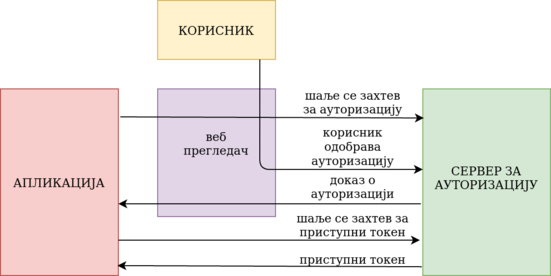
\includegraphics[scale=0.7]{slike/oauth2.png}
  \caption{Процес ауторизације код OAuth 2 протокола}
  \label{fig:oauth2}
\end{figure}

\subsection{Docker}
Docker је платформа дизајнирана тако да олакша процес креирања, упошљавања и покретања апликација употребом софтверских контејнера. Контејнери омогућавају програмерима да упакују апликацију, библиотеке и све остале зависности заједно у форми пакета. На овај начин се онемогућавају потенцијални проблеми да софтвер на једној машини ради, а на другој не, или да само делимично ради. У секцији \ref{hostovanjeservisa} је већ речено да су контејнери доста слични виртуелним машинама, али да имају нешто слабији степен виртуелизације, што им омогућава да буду ефикаснији. Контејнери су изоловани једни од других, и могу да комуницирају једни са другима кроз добро дефинисане канале комуникације.

Docker се састоји од клијентске и серверске апликације. Сва интеракција, укључујући покретање и заустављање контејнера, се обавља посредством клијентске апликације која комуницира са сервером. Основни концепти које Docker користи су слика (енг.~\textit{Docker image}), контејнер и сервис.

Слика представља шаблон, односно упутство како се креира контејнер. Паковање апликације и њених зависности у пакет подразумева изградњу слике; процес изградње описује се такозваним Docker датотекама (енг.~\textit{Dockerfile}), где се наводе кораци од којих се изградња састоји. Сама синтакса језика којим се описују ови кораци је слична синтакси Unix љуске (енг.~\textit{Unix shell}). Скоро свака Docker слика се састоји од слојева, где је сваки од слојева настао као пропратни ефекат извршавања корака за изградњу; једини изузетак су тзв. базне слике (енг.~\textit{base image}), које немају слојеве испод себе. Разлог овакве организације је то што изменом једног од корака изградње неке слике није потребно извршити поновну изградњу целе слике, већ само почевши од корака који се изменио.

Контејнер представља конкретан процес у меморији, и покреће се навођењем конкретне слике која ће представљати шаблон за његово креирање. Покретањем контејнера, на постојеће слојеве слике се додаје нови слој у који је могуће уписивати податке, а који ће контејнер користити током свог извршавања. Овај слој је обично јако танак, зато што контејнери у њега уписују само измене у односу на слојеве испод; биће уписане нове датотеке, информације о обрисаним датотекама, и измене постојећих датотека из нижих слојева.

Docker сервиси омогућавају контејнерима да се скалирају између више Docker сервера, чиме се добија скуп Docker сервера (енг.~\textit{swarm}) који међусобно сарађују употребом Docker интерфејса за програмирање апликација (енг.~\textit{Docker API}). Развијена је и алатка Docker Compose\cite{DockerCompose}, чији је циљ да олакша процес управљања и оркестрирања контејнерима развијеног софтверског система.

\section{Развој микросервисне апликације \textit{My Running Buddy}}

\chapter{Закључак}

\literatura

% \backmatter

\end{document} 
